\documentclass{article}

\usepackage{graphicx}
\usepackage{tikz}
\usepackage{tikzsymbols}
\usetikzlibrary{calc,patterns,shapes.geometric}
\pagestyle{empty}
\usepackage[margin=0pt]{geometry}
\geometry{papersize={14in,12in}}

\def\centerarc[#1](#2)(#3:#4:#5){\draw[#1] ($(#2)+({#5*cos(#3)},{#5*sin(#3)})$) arc (#3:#4:#5);}

\begin{document}
	\begin{figure}
		\centering
		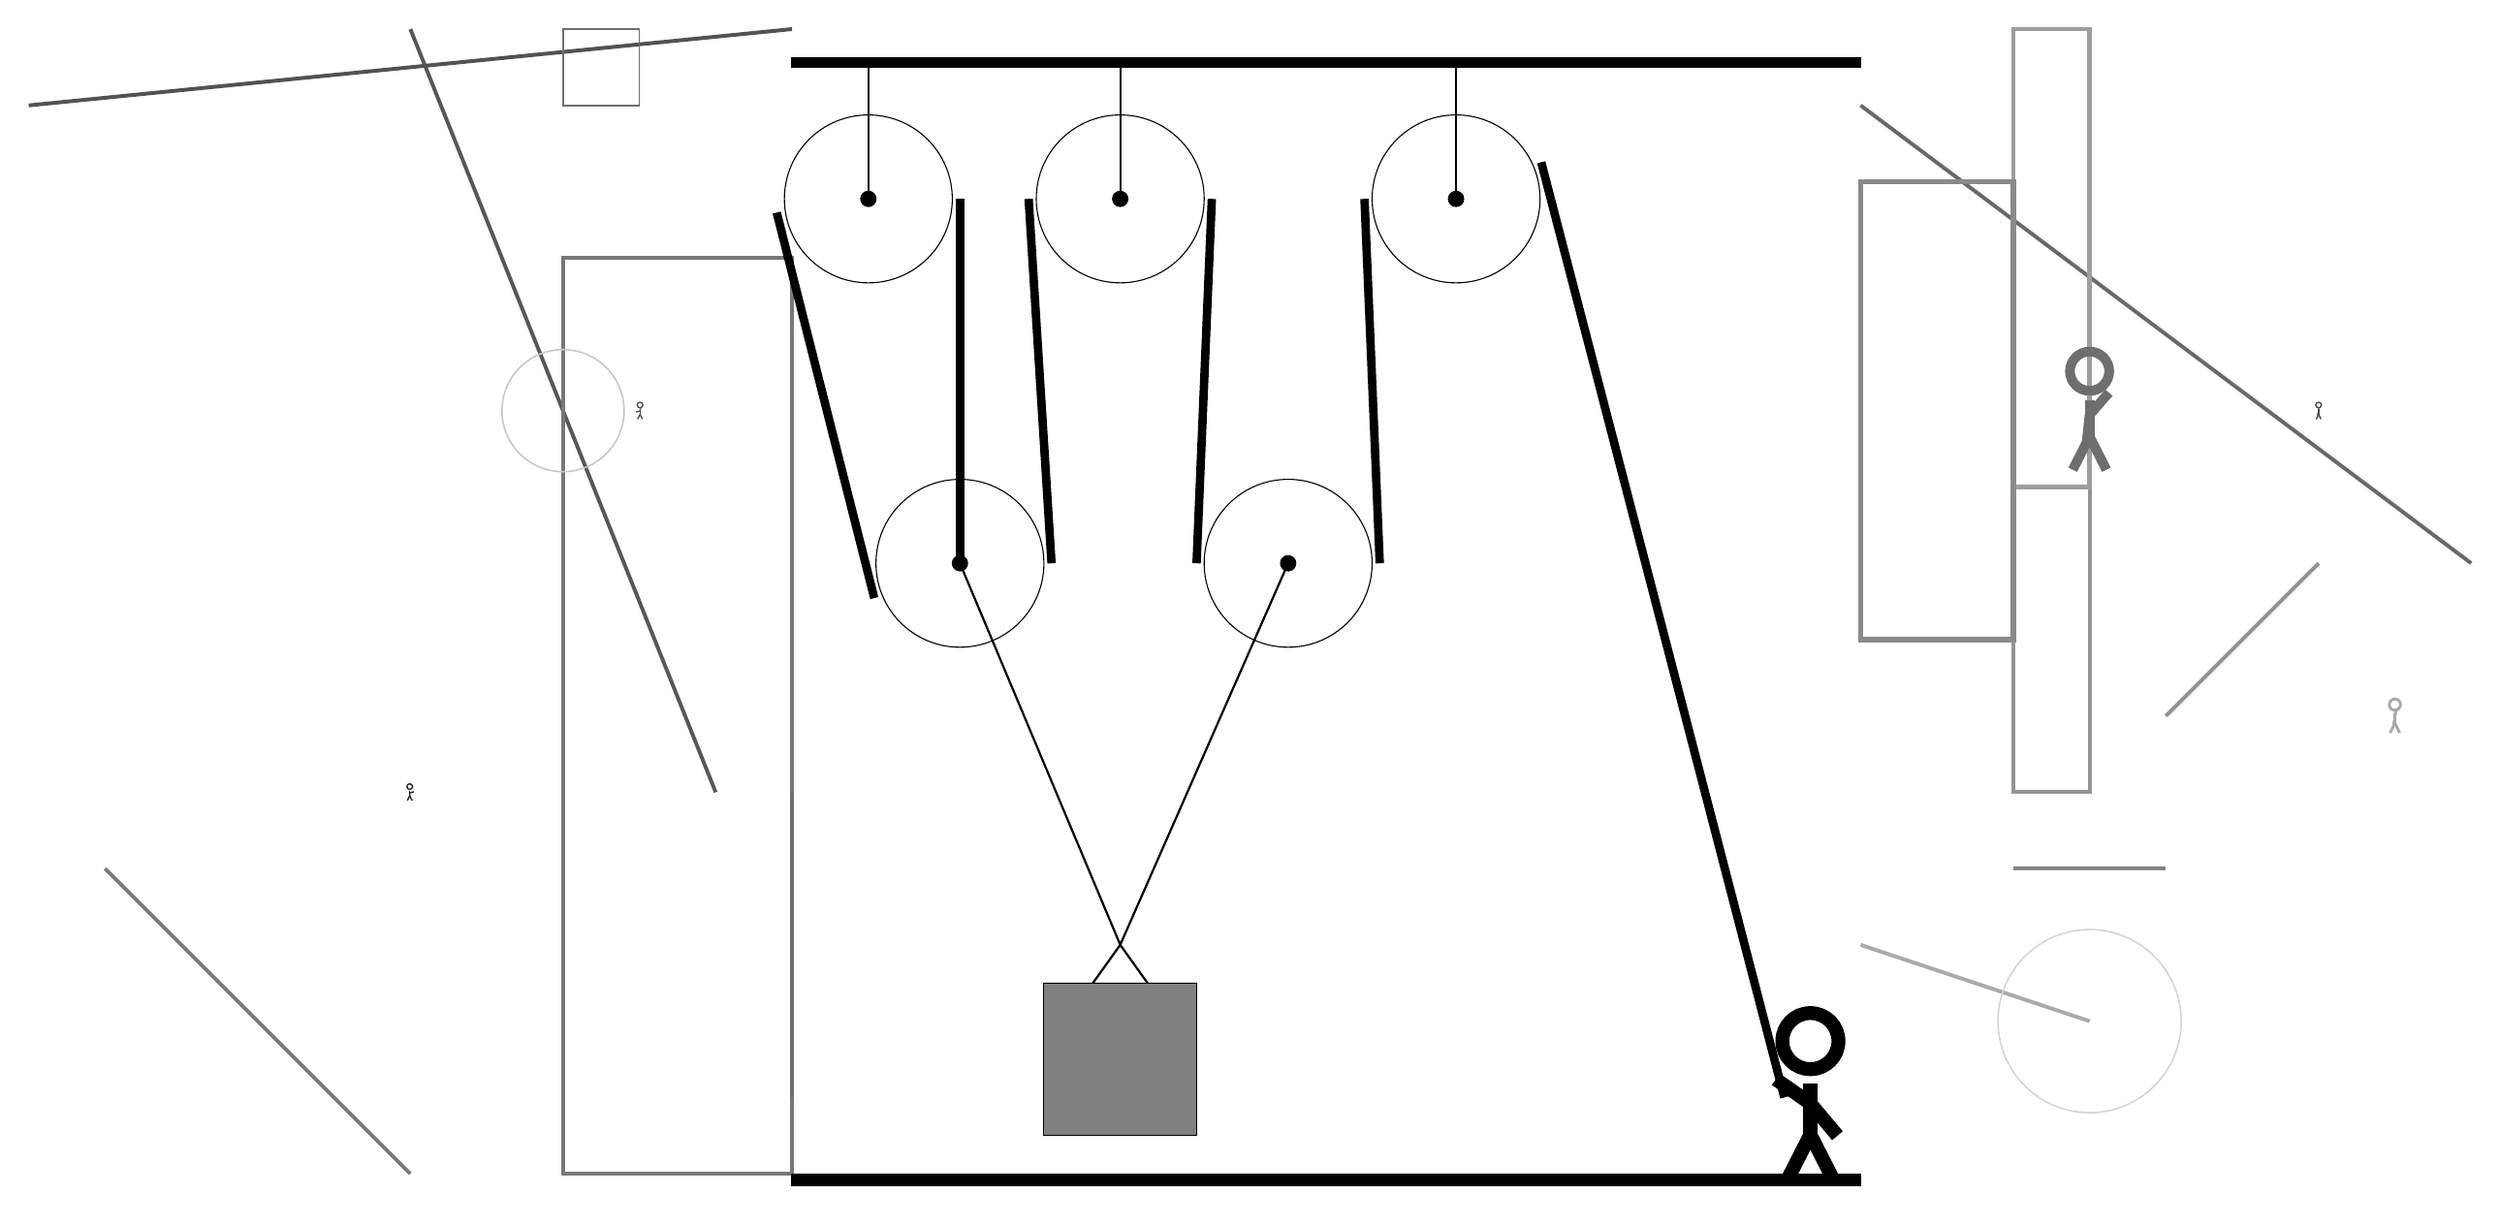
\begin{tikzpicture}
			%%%%% START %%%%%
			
			\draw[fill=black] (-2, 11.5) rectangle (12, 11.625);
			
			\draw (-1, 9.775) circle (1.1);
			\draw[fill=black] (-1, 9.775) circle (0.1);
			\draw[thick] (-1, 9.775) -- (-1, 11.5);
			
			\draw (2.3, 9.775) circle (1.1);
			\draw[fill=black] (2.3, 9.775) circle (0.1);
			\draw[thick] (2.3, 9.775) -- (2.3, 11.5);
			
			\draw[line width=0.5mm, color=black!33](15, -1) -- (12, 0);
			
			\draw[line width=0.5mm, color=black!66](-7, 12) -- (-3, 2);
			\draw[line width=0.5mm, color=black!53] (-2, 9) rectangle (-5, -3);
			\draw[line width=0.5mm, color=black!68](-2, 12) -- (-12, 11);
			
			\draw [line width=0.2mm, color=black!22](-5, 7) circle (0.8);
			
			\draw[line width=0.4mm, color=black!56] (-2, 2) rectangle (-2, -2);
			\node[line width=0.2mm, color=black!68] at (-4, 7) {\Strichmaxerl[1][7][81]};
			\draw[line width=0.5mm, color=black!59](12, 11) -- (20, 5);
			\draw[line width=0.5mm, color=black!42] (14, 2) rectangle (15, 6);
			\draw[line width=0.6mm, color=black!38] (14, 6) rectangle (15, 12);
			\node[line width=0.5mm, color=black!85] at (-7, 2) {\Strichmaxerl[1][89][13]};
			\draw[line width=0.5mm, color=black!52](-7, -3) -- (-11, 1);
			\node[line width=0.2mm, color=black!57] at (15, 7) {\Strichmaxerl[7][84][49]};
			
			\draw[line width=0.5mm, color=black!43](16, 3) -- (18, 5);
			\draw[line width=0.2mm, color=black!57] (-4, 11) rectangle (-5, 12);
			\node[line width=0.4mm, color=black!34] at (19, 3) {\Strichmaxerl[2][81][81]};
			
			\draw[line width=0.7mm, color=black!46] (12, 10) rectangle (14, 4);
			\draw[line width=0.5mm, color=black!48](16, 1) -- (14, 1);
			\draw [line width=0.2mm, color=black!17](15, -1) circle (1.2);
			\node[line width=0.4mm, color=black!70] at (18, 7) {\Strichmaxerl[1][75][87]};
			
			\draw (6.7, 9.775) circle (1.1);
			\draw[fill=black] (6.7, 9.775) circle (0.1);
			\draw[thick] (6.7, 9.775) -- (6.7, 11.5);
			
			\draw (0.2, 5) circle (1.1);
			\draw[fill=black] (0.2, 5) circle (0.1);
			
			\draw (4.5, 5) circle (1.1);
			\draw[fill=black] (4.5, 5) circle (0.1);
			
			\draw[thick] (0.2, 5) -- (2.3, 0)  -- (4.5, 5);
			\draw[thick]  (1.8, -0.7) -- (2.3, 0) -- (2.8, -0.7);
			\draw[fill=black!50] (1.3, -0.5) rectangle (3.3, -2.5);
			
			\draw[line width=1.1mm] (0.2, 5) -- (0.2, 9.775);
			\centerarc[line width=1.1mm](-1, 9.775)(0:200:1.2000000000000002);
			\draw[line width=1.1mm] (-2.2, 9.595) -- (-0.922, 4.544);
			\centerarc[line width=1.1mm](0.2, 5)(200:360:1.2000000000000002);
			\draw[line width=1.1mm](1.4, 5) -- (1.1, 9.775);
			\centerarc[line width=1.1mm](2.3, 9.775)(0:180:1.2000000000000002);
			\draw[line width=1.1mm] (3.5, 9.775) -- (3.3, 5);
			\centerarc[line width=1.1mm](4.5, 5)(180:360:1.2000000000000002);
			\draw[line width=1.1mm] (5.7, 5) -- (5.5, 9.775);
			\centerarc[line width=1.1mm](6.7, 9.775)(20:180:1.2000000000000002);
			\draw[line width=1.1mm](7.816, 10.255)  -- (11, -2);
			
			\node at (11.3, -2) {\Strichmaxerl[10][-35][-50]};
			
			\draw[fill=black] (-2, -3) rectangle (12, -3.15);
			
			%%%%% END %%%%%
		\end{tikzpicture}
	\end{figure}	
\end{document}